\subsection{Hiperkolumna}
\label{hypercolumn}

Patrząc na odzyskiwanie konturów z obrazu różnymi metodami w końcu trafi się na perspektywę, która będzie wywodziła się bezpośrednio z kory wzrokowej. Praca \cite{Curulku} przedstawia szczególny punkt widzenia w kwestii szukania krawędzi w obrazie, można w niej przeczytać o hiperkolumnie, o której wspomniane było w części \ref{v1}. Praca ta mimo, że opisuje tylko pewien model, może przedstawiać dobry pomysł na realizację zadania odzyskiwania konturów w postaci zbliżonej do tych, które są w korze wzrokowej człowieka.\\

\begin{figure}[ht]
	\centering
	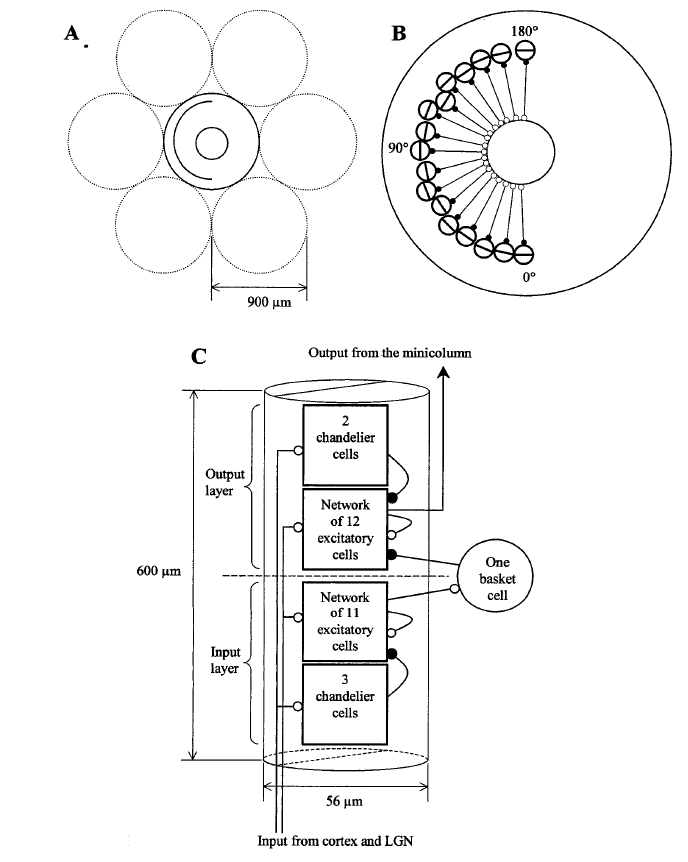
\includegraphics[width=.75\textwidth]{images/Hypercolumn.png}
	\caption{Model hiperkolumny, zaproponowany przez autorów pracy \cite{Curulku}, powstały na podstawie badań kory wzrokowej kota.}
	\label{fig:hypercolumn_model}
\end{figure}

%http://www.informaworld.com/smpp/content~db=all~content=a713663429
%%%Receptors can be classified broadly as excitatory (causing an increase in firing rate), inhibitory (causing a decrease in firing rate), or modulatory (causing long-lasting effects not directly related to firing rate).
Autorzy proponują, aby każdemu obszarowi w obrazie odpowiadała pewna hiperkolumna (rysunek \ref{fig:hypercolumn_model}A) składająca się z 17 różnie ukierunkowanych krawędzi (rysunek \ref{fig:hypercolumn_model}B), które są połączone w ramach tej kolumny w sieć BCPNN\footnote{Bayesian Confidence Propagation Neural Network -- Sieć neuronowa zbudowana na podstawie sieci Bayesowskiej.} mającej za zadanie wybrać spośród 17 krawędzi będących pod różnymi kątami tą najbardziej odpowiednią. Kolumna ta składa się z dwóch warstw (rysunek \ref{fig:hypercolumn_model}C), wejściowej i wyjściowej, w których łącznie 28 neuronów. Nie ma fizycznych połączeń między tymi dwoma warstwami innych niż poprzez jedną komórkę którą autorzy nazwali koszykiem\footnote{Z języka angielskiego -- basket cell.}. Komórka ta pełni rolę inhibitora -- czyli powoduje osłabienie sygnału wyjściowego z neuronów\footnote{W literaturze angielskojęzycznej spotyka się określenie firing rate -- które nie do końca szczęśliwie, ale jest w tej pracy tłumaczone na siłę sygnału wyjściowego. Jest to jednak tylko przeniesienie języka sztucznej inteligencji do stricte biologicznego opisu.}. Połączona jest natomiast z ekscytatorami, czyli komórkami, które powodują wzmocnienie sygnału wyjściowego z neuronów. Wszystkie neurony warstwy wejściowej są połączone z komórką koszykową, przez co mają na nią bezpośredni wpływ. Podobnie z komórkami warstwy wyjściowej, których wejścia sterowane są jedynie z łączącej obie warstwy komórki koszykowej. Dodatkowo w każdej warstwie kolumny znajdują się inhibitory, których zadaniem jest wpływanie na ekscytatory. Widać wyraźnie, że wyjściem z hiperkolumny jest sygnał z ekscytatorów warstwy wyjściowej. Natomiast samo wejście jest przekazywane z ciała kolankowatego bocznego.\\

Opis ten można by kontynuować wprowadzając więcej czysto biologicznych szczegółów. Autor tego dokumentu chciał jednak wprowadzając ten model pokazać z jednej strony, jak interpretowane mogą być odkrycia opisywane w części \ref{v1} tej pracy, z drugiej natomiast przedstawić pewną strukturę, która jest wykorzystywana w kilku kolejnych podejściach stosowanych głównie do symulacji działania pierwszorzędowej kory wzrokowej.


